%(BEGIN_QUESTION)
% Copyright 2009, Tony R. Kuphaldt, released under the Creative Commons Attribution License (v 1.0)
% This means you may do almost anything with this work of mine, so long as you give me proper credit

A process used in the oil refining industry to make high-octane gasoline feedstock is called {\it alkylation}.  So-called ``alky'' units employ a concentrated acid as the catalyst for the alkylation reaction, usually sulfuric acid:

$$\includegraphics[width=15.5cm]{i04139x01.eps}$$

The ``acid settler'' vessel is a separator, allowing the reaction products and acid catalyst to separate according to their respective densities (concentrated sulfuric acid being denser than any hydrocarbon).  The interface level between hydrocarbon liquid and acid must be tightly controlled for the process to work well.  It is bad for acid to ``carry over'' to the caustic scrubber (if the interface rises too high), and it is also bad for hydrocarbon liquids to leave the system through the ``reject acid'' line (if the interface falls too low).

\vskip 10pt

The major problem here is that the sulfuric acid is highly corrosive, creating a challenge for interface level measurement.  Identify a few different level-measurement technologies that might be appropriate for sensing the settler's interface level.

\vskip 20pt \vbox{\hrule \hbox{\strut \vrule{} {\bf Suggestions for Socratic discussion} \vrule} \hrule}

\begin{itemize}
\item{} By contrast, can you think of some level-measurement technologies that would {\it not} be appropriate for highly corrosive solutions?
\item{} Identify some of the different {\it flowmeter} technologies appropriate to various process lines shown for this alkylation unit.
\item{} What types of {\it personal protective equipment} (PPE) do you think an instrument technician might need to wear before working on a instrument contacting this highly concentrated acid?
\item{} How much fresh acid needs to be sent to the reactor, compared to the hydrocarbon feed rate?  Explain your answer based on what a {\it catalyst} does in a chemical reaction.
\item{} Older alkylation units used {\it hydrofluoric acid} instead of sulfuric acid because HF is a more effective catalyst for the alkylation reaction than H$_{2}$SO$_{4}$.  Unfortunately, while sulfuric acid at this concentration is quite dangerous, hydrofluoric acid is far worse.  HF tends to penetrate skin easier than many other acids, and when inside the body it dissolves bones!  Explain why the first-aid for topical HF exposure is to apply (or sometimes inject) a calcium gluconate (C$_{12}$H$_{22}$CaO$_{14}$) solution.
\end{itemize}

\underbar{file i04139}
%(END_QUESTION)





%(BEGIN_ANSWER)


%(END_ANSWER)





%(BEGIN_NOTES)

Bubbler systems (using plastic or ceramic dip tubes), non-contact radar, ultrasonic, weight, and nuclear (radiation) are all viable alternatives.

%INDEX% Measurement, level: strong acid/caustic solutions
%INDEX% Process: petroleum alkylation 

%(END_NOTES)


